\subsection{Visualization}

The results of the system is visualized in rviz, which is a 3D visualization tool for ROS. 

\subsubsection{Robot}
The data received from the controller are the joint states.
The visualizer, RViz, uses these states when determining the robots pose.
The robots construction is predefined and RViz only requires the joint states to draw the robot.
The length between the nodes and its appearance was provided by developer, in mesh format.

\begin{figure}[H]
\begin{center}
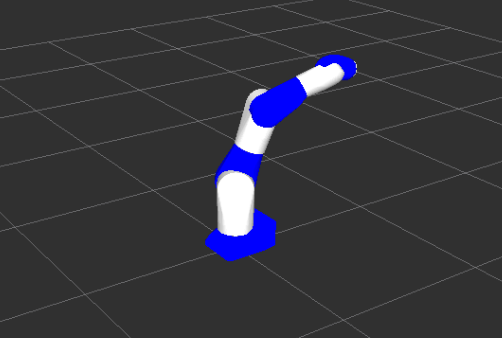
\includegraphics[width=12 cm]{robot}
\caption{3D-model of robot.}

\end{center}
\end{figure}

\subsubsection{Objects}
The objects in the image that the tracking algorithm considers being real moving objects are visualized. They are published as point clouds so that Rviz can subscribe to them and visualize them. If the tracking algorithm believes that an object has disappeared because of non-movement, it keeps the last seen point cloud of the object i.e. static objects in the scene are objects that the system thinks are standing still. 

\begin{figure}[H]
\begin{center}
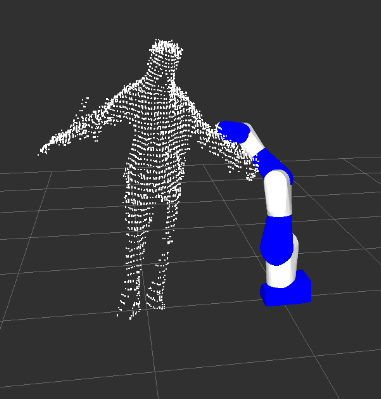
\includegraphics[width=12 cm]{humanandrobot}
\caption{Clustered object beside the robot.}

\end{center}
\end{figure}

\begin{figure}[H]
\begin{center}
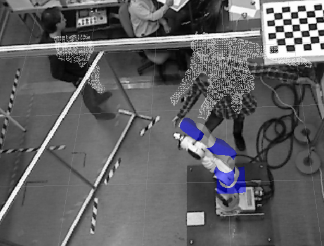
\includegraphics[width=12 cm]{humanandrobotinworld2}
\caption{Clustered objects and robot placed in world coordinate system.}

\end{center}
\end{figure}  

\subsubsection{Distances}
To visualize the resulting state of the system (the current safety zone) a line between the closest object and the closest joint of the robot is drawn. This line switches color depending on which state the system is in. The color of the line is thereby the result of the system. 

\begin{itemize}
  \item Red - Emergency zone
  \item Yellow - Safety zone 1 
  \item Green - Safety zone 2
  \item No line - Outside safety zone 2 
\end{itemize}

//lägg in en bild på hela systemet

